% ------------------------------------------------------------------------------
% TYPO3 CMS 7.0 - What's New - Chapter "Backend User Interface" (English Version)
%
% @author	Michael Schams <schams.net>
% @license	Creative Commons BY-NC-SA 3.0
% @link		http://typo3.org/download/release-notes/whats-new/
% @language	English
% ------------------------------------------------------------------------------
% LTXE-CHAPTER-UID:		39da62cf-7cf0e9ad-c4513cfe-f22835c9
% LTXE-CHAPTER-NAME:	Backend User Interface
% ------------------------------------------------------------------------------
% LTXE-SLIDE-START
% LTXE-SLIDE-UID:		fcbdd27c-e9005dff-0f4dd846-000ea412
% LTXE-SLIDE-TITLE:		In General
% LTXE-SLIDE-REFERENCE:	https://forge.typo3.org/issues/62333
% LTXE-SLIDE-REFERENCE:	https://forge.typo3.org/issues/62995
% LTXE-SLIDE-REFERENCE:	https://forge.typo3.org/issues/62158
% LTXE-SLIDE-REFERENCE:	https://forge.typo3.org/issues/61454
% ------------------------------------------------------------------------------

\begin{frame}[fragile]
	\frametitle{Backend User Interface}
	\framesubtitle{In General}

	\begin{itemize}
		\item Significant visual changes of the backend user interface
		\item Based on Twitter Bootstrap version 3.2.x
		\item All icons have been recreated and are in "tile" style now
		\item Icons use Font Awesome version 4.2.x
		\item Function menu left-hand-side has been adjusted accordingly
		\item Icons in the function menu use flat design, colourful background,
			monochrome/inverted pictogram in the foreground, rounded corners
		\item Width of function menu can be reduced to show icons only

	\end{itemize}

\end{frame}

% ------------------------------------------------------------------------------
% LTXE-SLIDE-START
% LTXE-SLIDE-UID:		0ae980b6-0d2ae6c6-52182f58-aaef69e3
% LTXE-SLIDE-TITLE:		Look & Feel (1)
% ------------------------------------------------------------------------------

\begin{frame}[fragile]
	\frametitle{Backend User Interface}
	\framesubtitle{Look \& Feel}

	\begin{figure}
		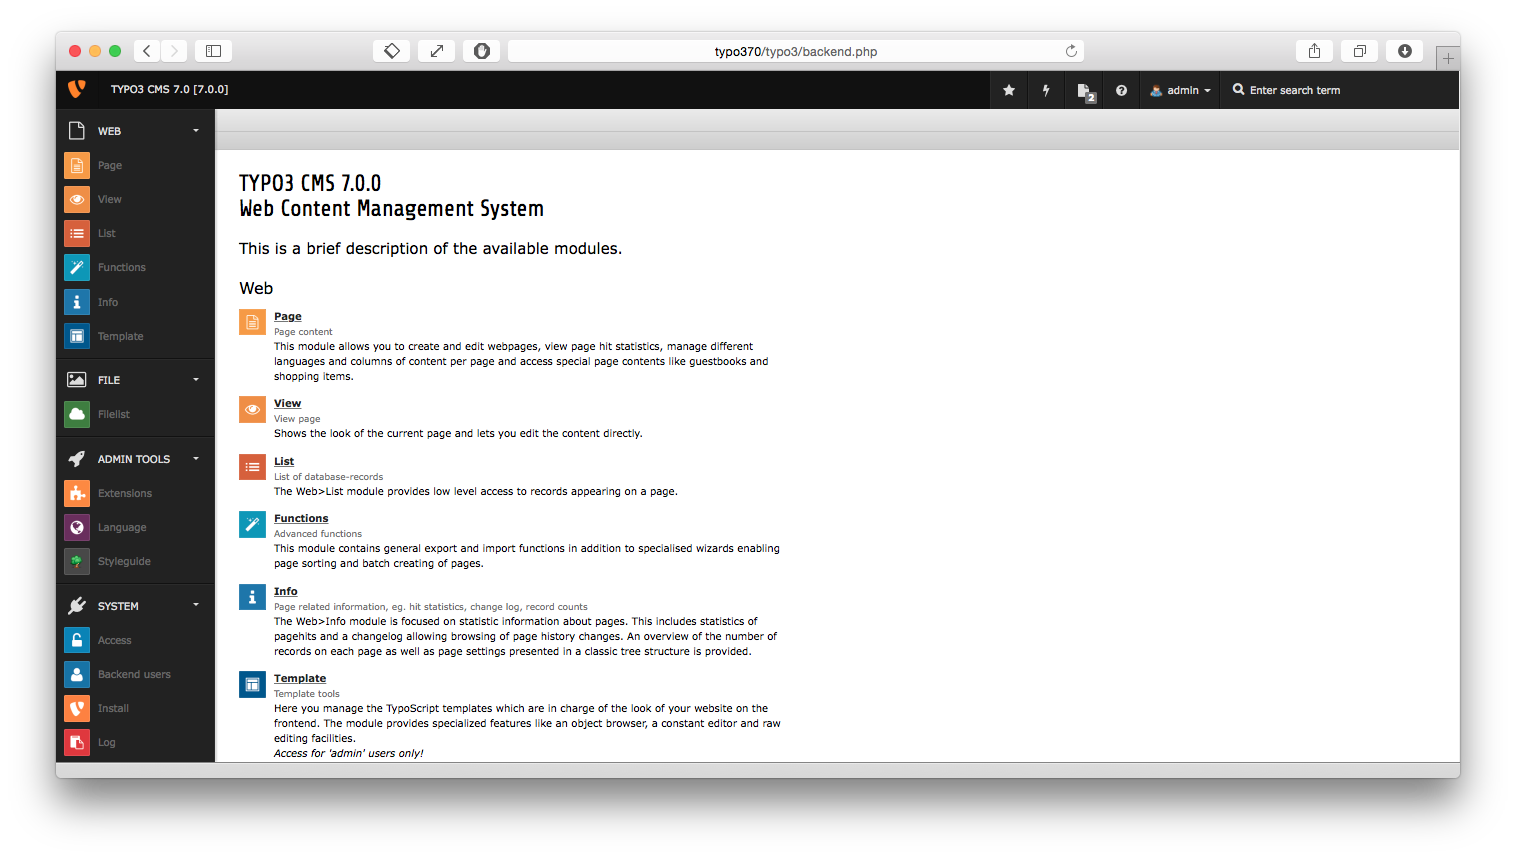
\includegraphics[width=0.90\linewidth]{BackendUserInterface/be-totalscreenshot1.png}
	\end{figure}

\end{frame}

% ------------------------------------------------------------------------------
% LTXE-SLIDE-START
% LTXE-SLIDE-UID:		250b123b-2c0bfce4-506f16b0-629baa10
% LTXE-SLIDE-TITLE:		Look & Feel (2)
% ------------------------------------------------------------------------------

\begin{frame}[fragile]
	\frametitle{Backend User Interface}
	\framesubtitle{Look \& Feel}

	\begin{figure}
		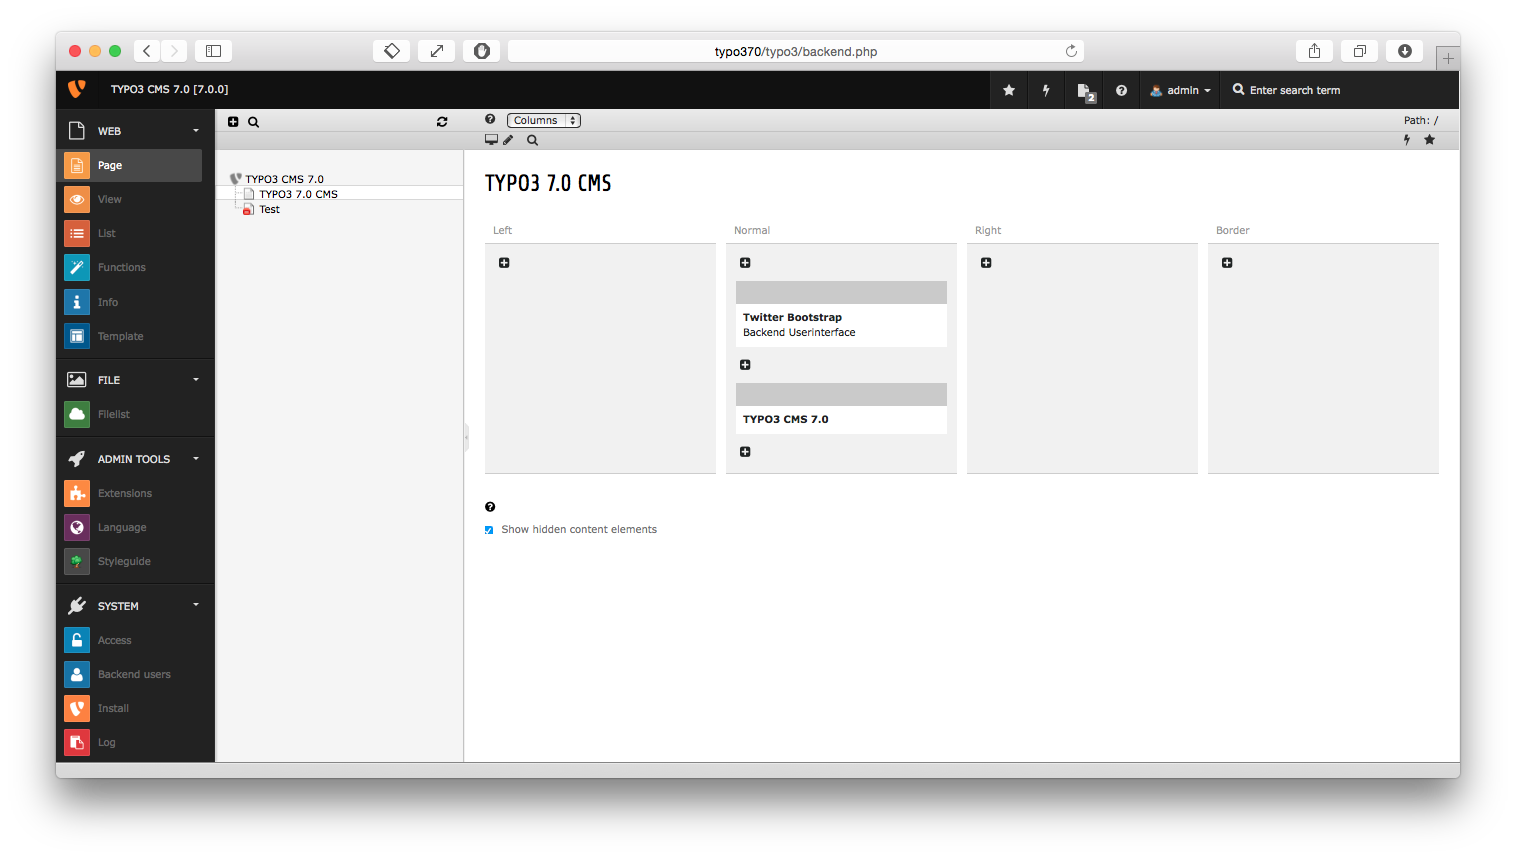
\includegraphics[width=0.90\linewidth]{BackendUserInterface/be-totalscreenshot2.png}
	\end{figure}

\end{frame}

% ------------------------------------------------------------------------------
% LTXE-SLIDE-START
% LTXE-SLIDE-UID:		2d4d33ee-071ae6ed-9f4d0c04-49361364
% LTXE-SLIDE-TITLE:		Look & Feel (3)
% ------------------------------------------------------------------------------

\begin{frame}[fragile]
	\frametitle{Backend User Interface}
	\framesubtitle{Look \& Feel}

	\begin{figure}
		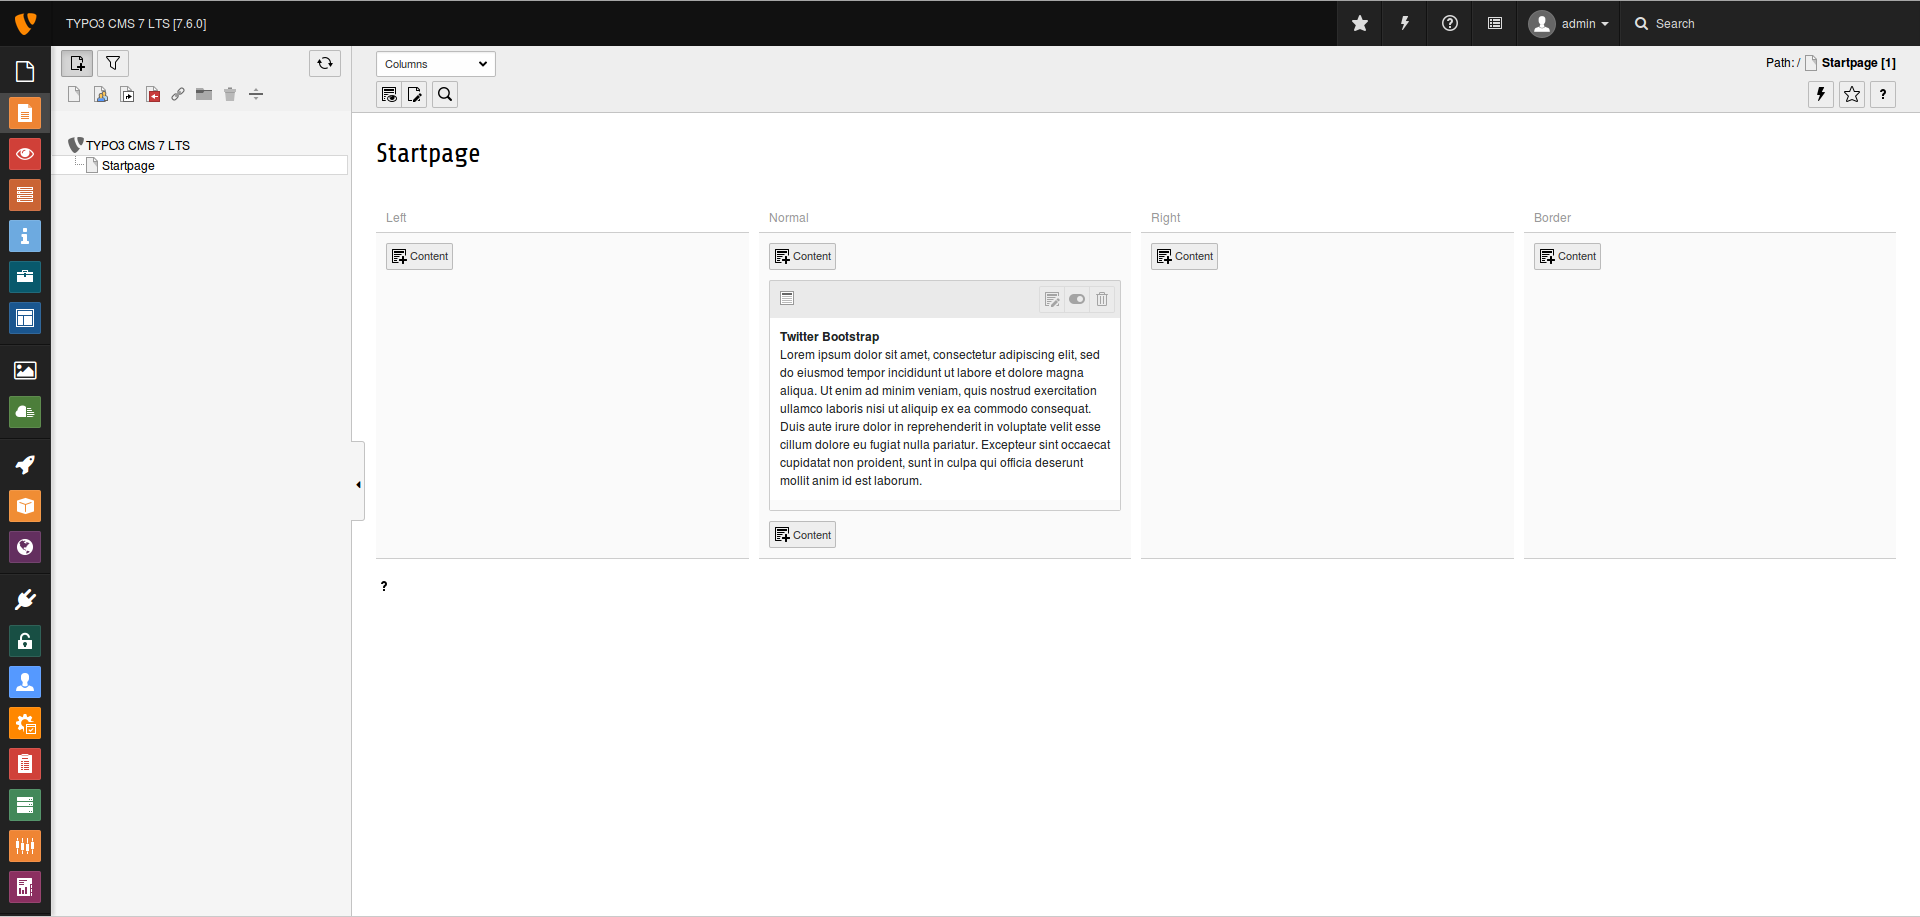
\includegraphics[width=0.90\linewidth]{BackendUserInterface/be-totalscreenshot3.png}
	\end{figure}

\end{frame}

% ------------------------------------------------------------------------------
% LTXE-SLIDE-START
% LTXE-SLIDE-UID:		de58d070-98483f3d-0949f2d1-856a9e7e
% LTXE-SLIDE-TITLE:		Backend User Login
% ------------------------------------------------------------------------------

\begin{frame}[fragile]
	\frametitle{Backend User Interface}
	\framesubtitle{Backend User Login}

	\begin{figure}
		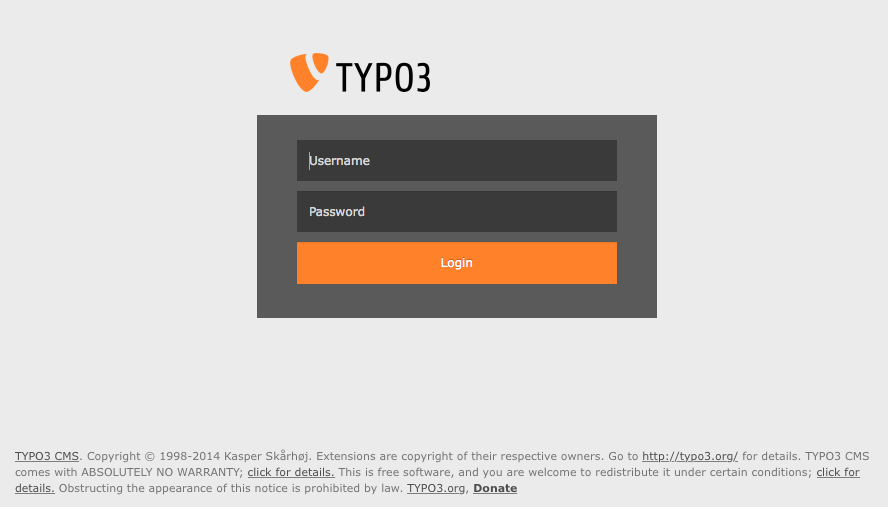
\includegraphics[width=0.80\linewidth]{BackendUserInterface/be-login.png}
	\end{figure}

\end{frame}

% ------------------------------------------------------------------------------
% LTXE-SLIDE-START
% LTXE-SLIDE-UID:		9baa13c8-78b2f416-28da8e3d-b234e7dc
% LTXE-SLIDE-TITLE:		Refactor & recolor Modul Menu (Bootstrap)
% LTXE-SLIDE-REFERENCE:	https://forge.typo3.org/issues/62353
% ------------------------------------------------------------------------------

\begin{frame}[fragile]
	\frametitle{Backend User Interface}
	\framesubtitle{Top Bar (Module Menu)}

	\begin{figure}
		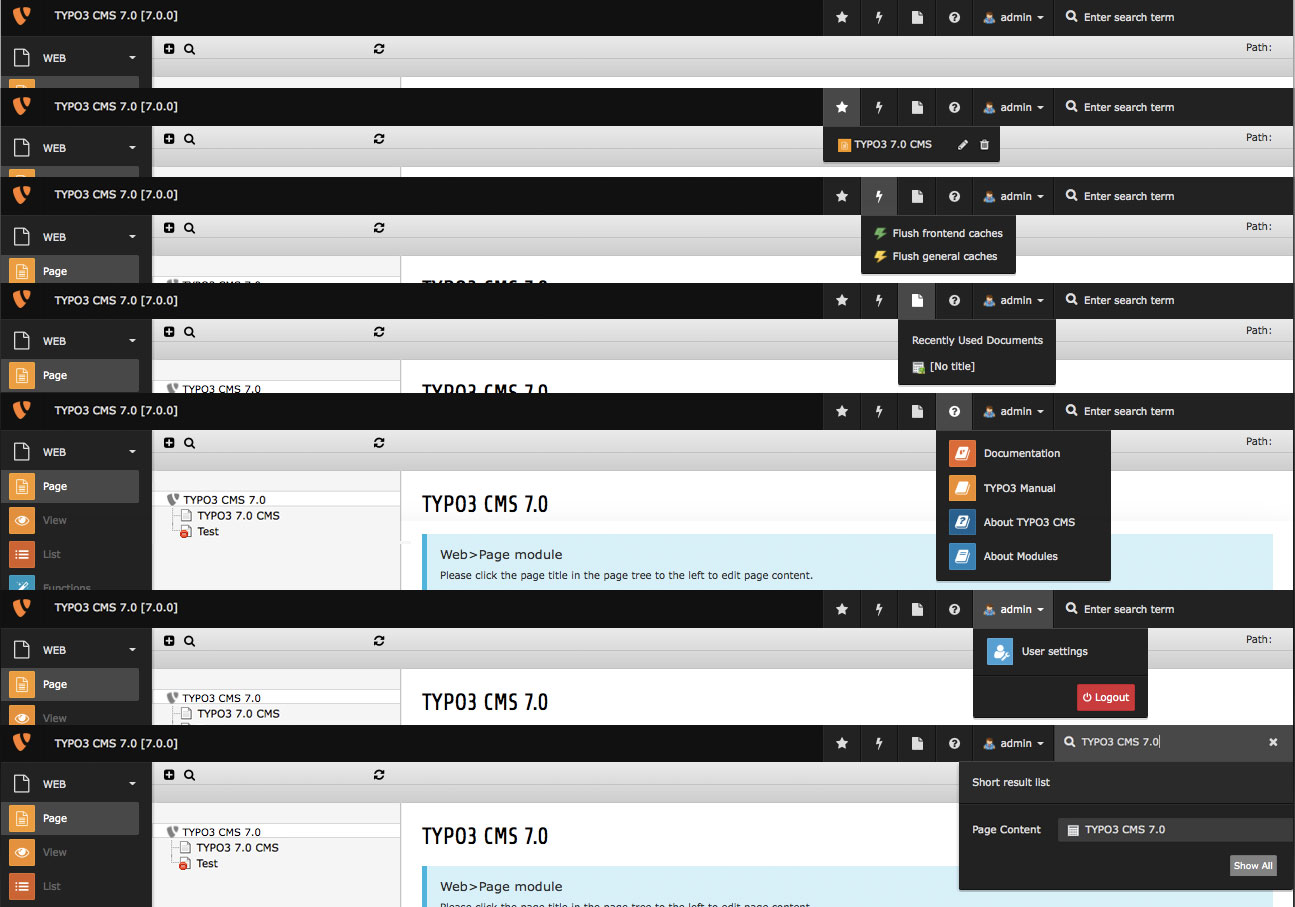
\includegraphics[width=0.70\linewidth]{BackendUserInterface/be-topbar.jpg}
	\end{figure}

\end{frame}

% ------------------------------------------------------------------------------
% LTXE-SLIDE-START
% LTXE-SLIDE-UID:		4369ae5e-948d1afa-8212cd72-c91c660b
% LTXE-SLIDE-TITLE:		New List Module Styling
% LTXE-SLIDE-REFERENCE:	https://forge.typo3.org/issues/62963
% ------------------------------------------------------------------------------

\begin{frame}[fragile]
	\frametitle{Backend User Interface}
	\framesubtitle{List Module and Clipboard}

	\begin{figure}
		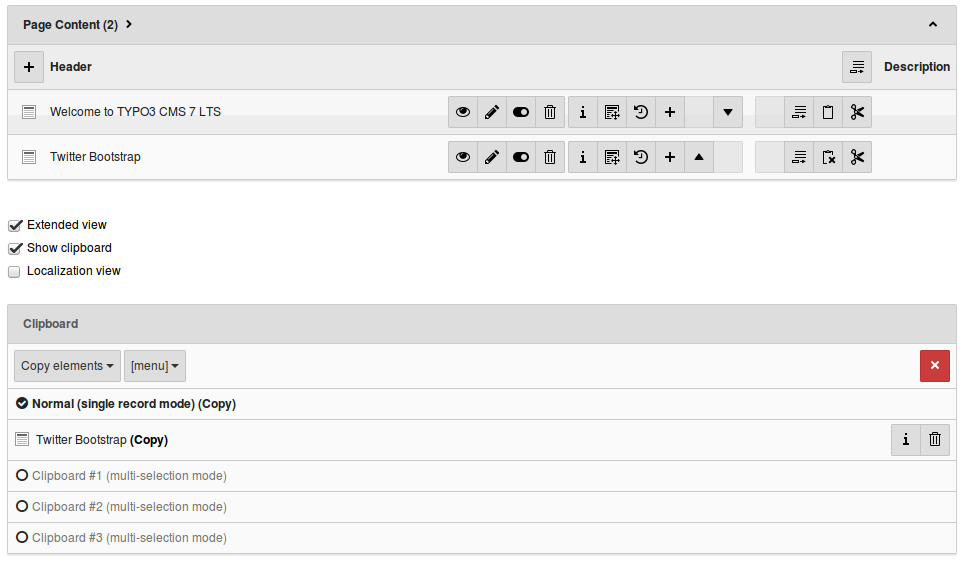
\includegraphics[width=0.80\linewidth]{BackendUserInterface/be-list.png}
	\end{figure}

\end{frame}

% ------------------------------------------------------------------------------
% LTXE-SLIDE-START
% LTXE-SLIDE-UID:		252361f7-e5c42ec2-a90ecd64-4331f02b
% LTXE-SLIDE-TITLE:		Table Style
% LTXE-SLIDE-REFERENCE:	https://forge.typo3.org/issues/62159
% ------------------------------------------------------------------------------

\begin{frame}[fragile]
	\frametitle{Backend User Interface}
	\framesubtitle{Table Style}

	\begin{figure}
		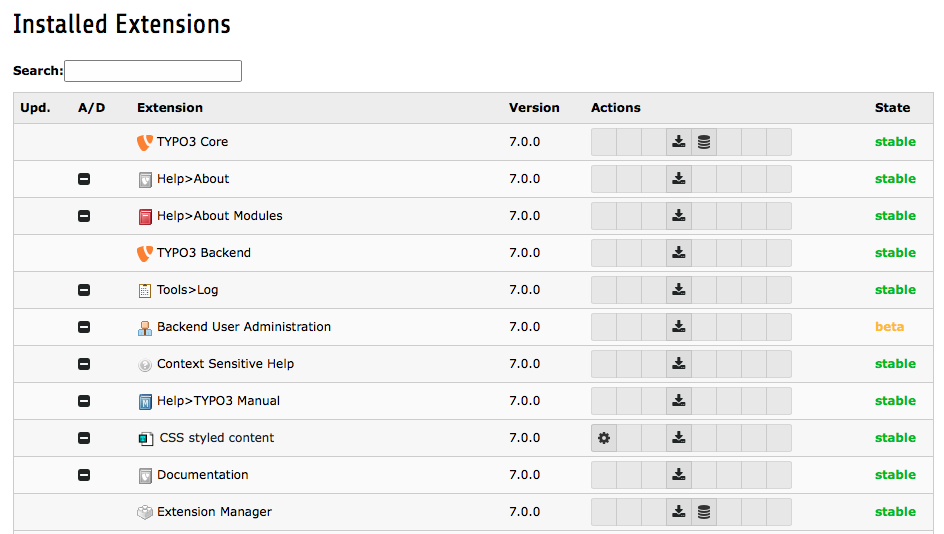
\includegraphics[width=0.99\linewidth]{BackendUserInterface/be-table.png}
	\end{figure}

\end{frame}

% ------------------------------------------------------------------------------
% LTXE-SLIDE-START
% LTXE-SLIDE-UID:		785f717d-a7c4d1dd-f186ca6a-060c1dc4
% LTXE-SLIDE-TITLE:		Page And List Search
% LTXE-SLIDE-REFERENCE:	https://forge.typo3.org/issues/59763
% ------------------------------------------------------------------------------

\begin{frame}[fragile]
	\frametitle{Backend User Interface}
	\framesubtitle{Search in List and Page View}

	\begin{itemize}
		\item Click on magnifying glass to show search bar in "list" and "page" view\newline
			(search function was at the end of the page before)
	\end{itemize}

	\begin{figure}
		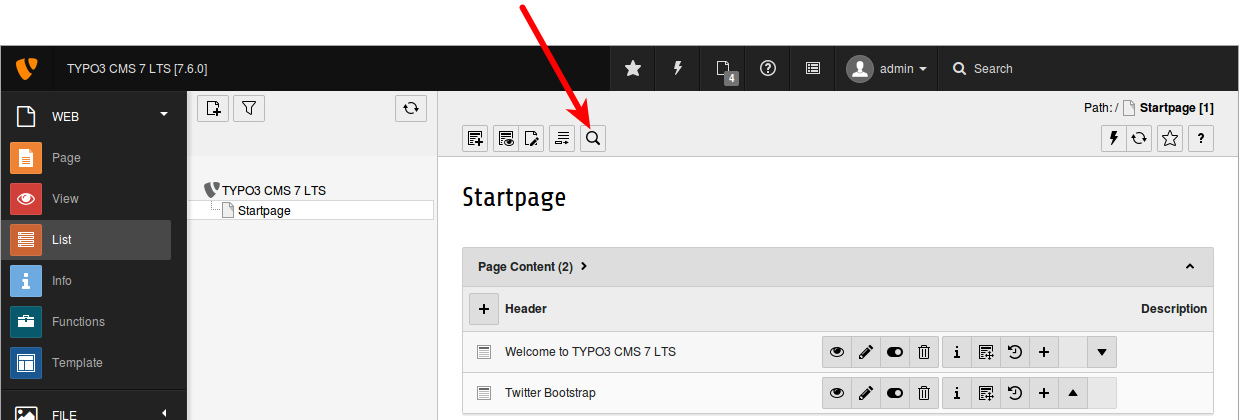
\includegraphics[width=0.95\linewidth]{BackendUserInterface/be-search.jpg}
	\end{figure}

\end{frame}

% ------------------------------------------------------------------------------
% LTXE-SLIDE-START
% LTXE-SLIDE-UID:		df97fbbf-9ea6c6a9-d9b4c5d4-f8fe1601
% LTXE-SLIDE-TITLE:		Migrate Counter of Open Documents to Bootstrap "Badge"
% LTXE-SLIDE-REFERENCE:	https://forge.typo3.org/issues/61675
% ------------------------------------------------------------------------------

\begin{frame}[fragile]
	\frametitle{Backend User Interface}
	\framesubtitle{Badge Shows Open Documents}

	\begin{itemize}
		\item Number of open documents are shown as a Bootstrap "badge"\newline
			(requires system extension "Open Documents")
	\end{itemize}
	\begin{figure}
		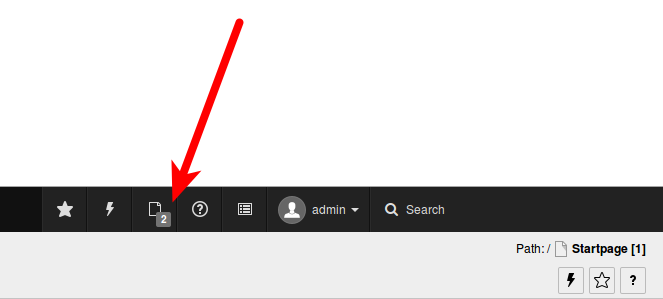
\includegraphics[width=0.75\linewidth]{BackendUserInterface/be-badge.png}
	\end{figure}

\end{frame}

% ------------------------------------------------------------------------------
% LTXE-SLIDE-START
% LTXE-SLIDE-UID:		a25faae4-8c12c45e-b337b64a-0cf2f53f
% LTXE-SLIDE-TITLE:		Rebrush FlashMessage
% LTXE-SLIDE-REFERENCE:	https://forge.typo3.org/issues/62580
% ------------------------------------------------------------------------------

\begin{frame}[fragile]
	\frametitle{Backend User Interface}
	\framesubtitle{Flash Messages}

	\begin{itemize}
		\item Visual appearance of Flash Messages has been updated
		\item Contrast of text vs box background colour improved
	\end{itemize}

	\begin{columns}[T]
		\begin{column}{.25\textwidth}
			\smaller\hfill
				\begingroup\color{typo3red}TYPO3 CMS < 7.0\endgroup
			\normalsize
		\end{column}

		\begin{column}{.5\textwidth}
			\begin{figure}\vspace*{-0.6cm}
				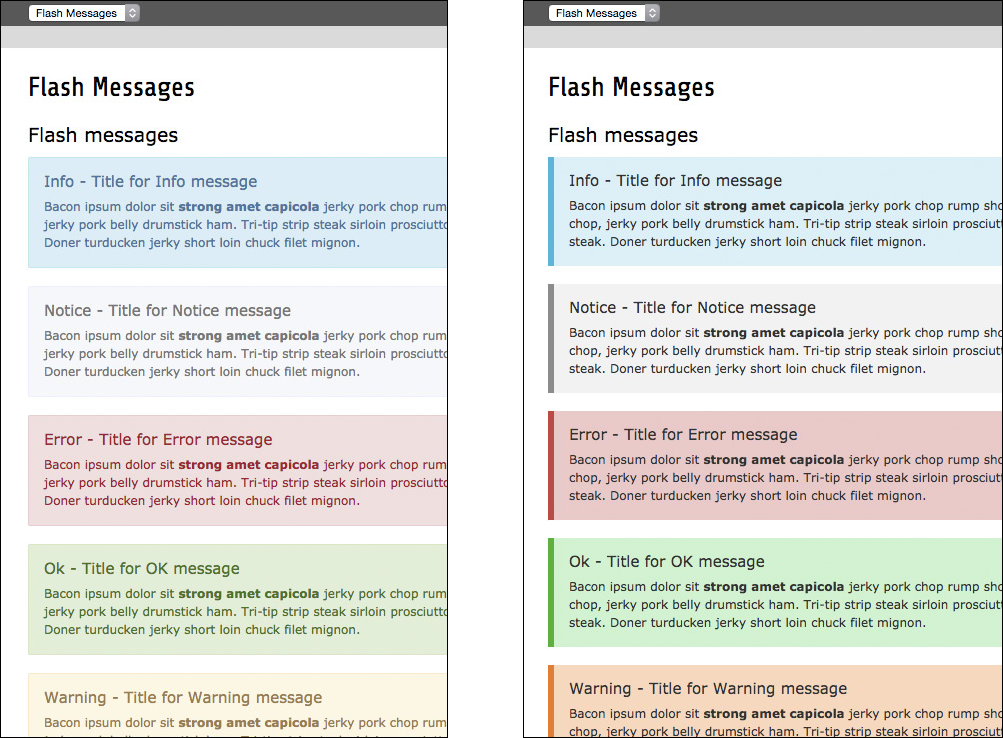
\includegraphics[width=0.99\linewidth]{BackendUserInterface/be-flashmessages.png}
			\end{figure}
		\end{column}

		\begin{column}{.25\textwidth}
			\smaller
				\begingroup\color{typo3red}TYPO3 CMS >= 7.0\endgroup
			\normalsize
		\end{column}
	\end{columns}

\end{frame}

% ------------------------------------------------------------------------------
% LTXE-SLIDE-START
% LTXE-SLIDE-UID:		d6a85376-8109aa8c-45a40582-7edb975a
% LTXE-SLIDE-TITLE:		Video Player in Info Window
% LTXE-SLIDE-REFERENCE:	https://forge.typo3.org/issues/61668
% ------------------------------------------------------------------------------

\begin{frame}[fragile]
	\frametitle{Backend User Interface}
	\framesubtitle{Video Player in Info Window}

	\begin{itemize}
		\item HTML5 audio and video files can be played in info window\newline
			(where meta data is shown)
	\end{itemize}

	\begin{figure}
		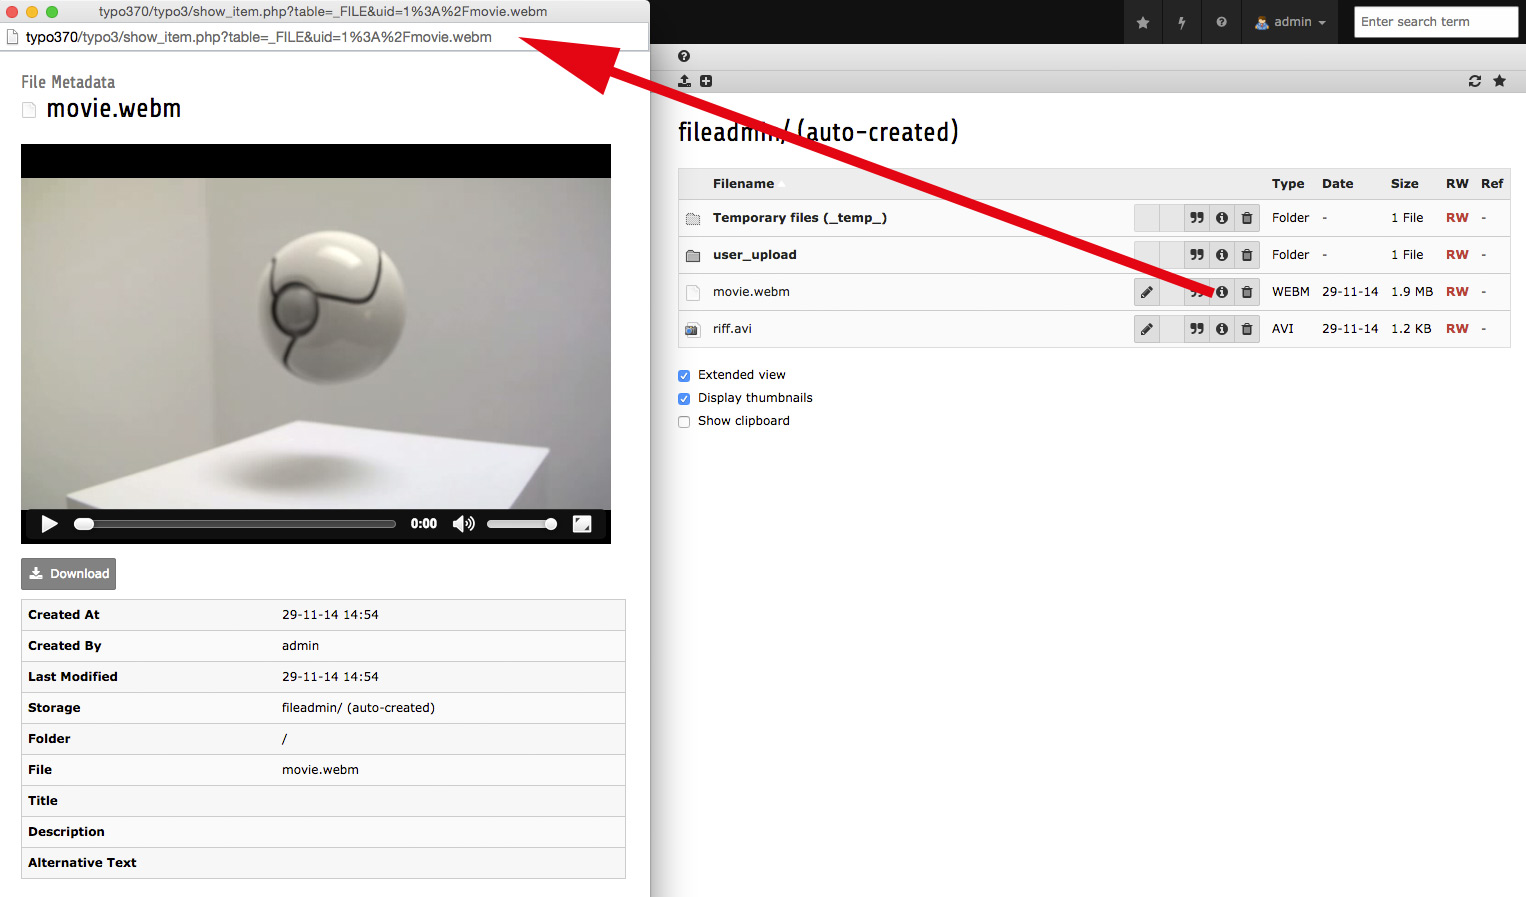
\includegraphics[width=0.70\linewidth]{BackendUserInterface/be-info.jpg}
	\end{figure}

\end{frame}

% ------------------------------------------------------------------------------
